%
% Common preamble for all three parts.
%
\usepackage[T1]{fontenc}
\usepackage[utf8]{inputenc}
\usepackage[catalan]{babel}
\usepackage{amsmath}
\usepackage{color}
\usepackage{minted}
\usepackage{hyperref}
\usepackage{multicol}
\usepackage{tabularx, booktabs}
\usepackage{tikz}

% only inline todonotes work
\usepackage{xkeyval}
\usepackage[textsize=small]{todonotes}
\presetkeys{todonotes}{inline}{}

\usetikzlibrary{shapes,arrows,positioning,shadows}

% no nav buttons
\usenavigationsymbolstemplate{}

\newcommand{\bftt}[1]{\textbf{\texttt{#1}}}
\newcommand{\comment}[1]{{\color[HTML]{008080}\textit{\textbf{\texttt{#1}}}}}
\newcommand{\cmd}[1]{{\color[HTML]{008000}\bftt{#1}}}
\newcommand{\bs}{\char`\\}
\newcommand{\cmdbs}[1]{\cmd{\bs#1}}
\newcommand{\lcb}{\char '173}
\newcommand{\rcb}{\char '175}
\newcommand{\cmdbegin}[1]{\cmdbs{begin\lcb}\bftt{#1}\cmd{\rcb}}
\newcommand{\cmdend}[1]{\cmdbs{end\lcb}\bftt{#1}\cmd{\rcb}}

\newcommand{\wllogo}{\textbf{Overleaf}}

% this is where the example source files are loaded from
% do not include a trailing slash
\newcommand{\fileuri}{https://raw.github.com/pastells/curs-latex/master/ca}

\newcommand{\wlserver}{https://www.overleaf.com}
\newcommand{\wlnewdoc}[1]{\wlserver/docs?snip\_uri=\fileuri/#1\&splash=none}

\def\tikzname{Ti\emph{k}Z}

% from http://tex.stackexchange.com/questions/5226/keyboard-font-for-latex
\newcommand*\keystroke[1]{%
  \tikz[baseline=(key.base)]
    \node[%
      draw,
      fill=white,
      drop shadow={shadow xshift=0.25ex,shadow yshift=-0.25ex,fill=black,opacity=0.75},
      rectangle,
      rounded corners=2pt,
      inner sep=1pt,
      line width=0.5pt,
      font=\scriptsize\sffamily
    ](key) {#1\strut}
  ;
}
\newcommand{\keystrokebftt}[1]{\keystroke{\bftt{#1}}}

% stolen from minted.dtx
\newenvironment{exampletwoup}
  {\VerbatimEnvironment
   \begin{VerbatimOut}{example.out}}
  {\end{VerbatimOut}
   \setlength{\parindent}{0pt}
   \fbox{\begin{tabular}{l|l}
   \begin{minipage}{0.55\linewidth}
     \inputminted[fontsize=\small,resetmargins]{latex}{example.out}
   \end{minipage} &
   \begin{minipage}{0.35\linewidth}
     \input{example.out}
   \end{minipage}
   \end{tabular}}}

\newenvironment{exampletwouptiny}
  {\VerbatimEnvironment
   \begin{VerbatimOut}{example.out}}
  {\end{VerbatimOut}
   \setlength{\parindent}{0pt}
   \fbox{\begin{tabular}{l|l}
   \begin{minipage}{0.55\linewidth}
     \inputminted[fontsize=\scriptsize,resetmargins]{latex}{example.out}
   \end{minipage} &
   \begin{minipage}{0.35\linewidth}
     \setlength{\parskip}{6pt plus 1pt minus 1pt}%
     \raggedright\scriptsize\input{example.out}
   \end{minipage}
   \end{tabular}}}

\newenvironment{exampletwouptinynoframe}
  {\VerbatimEnvironment
   \begin{VerbatimOut}{example.out}}
  {\end{VerbatimOut}
   \setlength{\parindent}{0pt}
   \begin{tabular}{l|l}
   \begin{minipage}{0.55\linewidth}
     \inputminted[fontsize=\scriptsize,resetmargins]{latex}{example.out}
   \end{minipage} &
   \begin{minipage}{0.35\linewidth}
     \setlength{\parskip}{6pt plus 1pt minus 1pt}%
     \raggedright\scriptsize\input{example.out}
   \end{minipage}
   \end{tabular}}

\title{Introducció Interactiva a \LaTeX}
\author{Pol Pastells}
\titlegraphic{%

\includegraphics[height=24pt]{overleaf} \quad

\includegraphics[height=24pt]{logo_UB.png}
}

\date{3 de maig de 2024}

\subtitle{Primera part}

\begin{document}

%%%%%%%%%%%%%%%%%%%%%%%%%%%%%%%%%%%%%%%%%%%%%%%%%%%%%%%%%%%%%%%%%%%%%%%%%%%%%%%
%%%%%%%%%%%%%%%%%%%%%%%%%%%%%%%%%%%%%%%%%%%%%%%%%%%%%%%%%%%%%%%%%%%%%%%%%%%%%%%
%%%%%%%%%%%%%%%%%%%%%%%%%%%%%%%%%%%%%%%%%%%%%%%%%%%%%%%%%%%%%%%%%%%%%%%%%%%%%%%
\begin{frame}
\titlepage
\end{frame}

%%%%%%%%%%%%%%%%%%%%%%%%%%%%%%%%%%%%%%%%%%%%%%%%%%%%%%%%%%%%%%%%%%%%%%%%%%%%%%%
%%%%%%%%%%%%%%%%%%%%%%%%%%%%%%%%%%%%%%%%%%%%%%%%%%%%%%%%%%%%%%%%%%%%%%%%%%%%%%%
%%%%%%%%%%%%%%%%%%%%%%%%%%%%%%%%%%%%%%%%%%%%%%%%%%%%%%%%%%%%%%%%%%%%%%%%%%%%%%%
\section{Fonaments}

\begin{frame}{Continguts}
\tableofcontents[currentsection]
\end{frame}

%%%%%%%%%%%%%%%%%%%%%%%%%%%%%%%%%%%%%%%%%%%%%%%%%%%%%%%%%%%%%%%%%%%%%%%%%%%%%%%
%%%%%%%%%%%%%%%%%%%%%%%%%%%%%%%%%%%%%%%%%%%%%%%%%%%%%%%%%%%%%%%%%%%%%%%%%%%%%%%
%%%%%%%%%%%%%%%%%%%%%%%%%%%%%%%%%%%%%%%%%%%%%%%%%%%%%%%%%%%%%%%%%%%%%%%%%%%%%%%
\subsection{Introducció}

\begin{frame}{Per què \LaTeX{}?}
\begin{itemize}
\item Fa documents amb una bona presentació
\begin{itemize}
\item Especialment per a matemàtiques i lingüística
\end{itemize}
%
\item Creat per científics, per a científics
\begin{itemize}
\item Una comunitat gran i activa
\end{itemize}
%
\item És potent --- podeu estendre-ho
\begin{itemize}
\item Paquets per a treballs, presentacions, tesis \dots
\end{itemize}
\end{itemize}
\end{frame}

%%%%%%%%%%%%%%%%%%%%%%%%%%%%%%%%%%%%%%%%%%%%%%%%%%%%%%%%%%%%%%%%%%%%%%%%%%%%%%%
%%%%%%%%%%%%%%%%%%%%%%%%%%%%%%%%%%%%%%%%%%%%%%%%%%%%%%%%%%%%%%%%%%%%%%%%%%%%%%%
%%%%%%%%%%%%%%%%%%%%%%%%%%%%%%%%%%%%%%%%%%%%%%%%%%%%%%%%%%%%%%%%%%%%%%%%%%%%%%%
\begin{frame}[fragile]{Com funciona?}
\begin{itemize}
\item Escriviu el document a \texttt{text pla} amb \cmd{ordres} que
descriuen la seva estructura i significat.
\item Usa ordres per descriure `el contingut', no `el format'.
\item El programa \texttt{latex} processa el text i les ordres per a produir un
document amb un format bonic.
\end{itemize}
\vskip 2ex
\begin{center}
\begin{minted}[frame=single]{latex}
La \textit{fonologia} estudia els \textbf{fonemes}.
\end{minted}
\vskip 2ex
\tikz\node[single arrow,fill=gray,font=\ttfamily\bfseries,%
  rotate=270,xshift=-1em]{latex};
\vskip 2ex
\fbox{La \textit{fonologia} estudia els \textbf{fonemes}.}
\end{center}
\end{frame}

%%%%%%%%%%%%%%%%%%%%%%%%%%%%%%%%%%%%%%%%%%%%%%%%%%%%%%%%%%%%%%%%%%%%%%%%%%%%%%%
%%%%%%%%%%%%%%%%%%%%%%%%%%%%%%%%%%%%%%%%%%%%%%%%%%%%%%%%%%%%%%%%%%%%%%%%%%%%%%%
%%%%%%%%%%%%%%%%%%%%%%%%%%%%%%%%%%%%%%%%%%%%%%%%%%%%%%%%%%%%%%%%%%%%%%%%%%%%%%%
\begin{frame}[fragile]{Exemples d'ordres i la seva sortida}
\begin{exampletwoup}
\begin{itemize}
\item Mel
\item Llet
\item Galetes
\end{itemize}
\end{exampletwoup}
\vskip 2ex
\begin{exampletwoup}
\begin{figure}

\includegraphics{gus}
\end{figure}
\end{exampletwoup}
\vskip 2ex
\begin{exampletwoup}
\begin{equation}
\alpha + \beta + 1
\end{equation}
\end{exampletwoup}

\end{frame}



%%%%%%%%%%%%%%%%%%%%%%%%%%%%%%%%%%%%%%%%%%%%%%%%%%%%%%%%%%%%%%%%%%%%%%%%%%%%%%%
%%%%%%%%%%%%%%%%%%%%%%%%%%%%%%%%%%%%%%%%%%%%%%%%%%%%%%%%%%%%%%%%%%%%%%%%%%%%%%%
%%%%%%%%%%%%%%%%%%%%%%%%%%%%%%%%%%%%%%%%%%%%%%%%%%%%%%%%%%%%%%%%%%%%%%%%%%%%%%%
\begin{frame}[fragile]{Començant}
\begin{itemize}
\item Un document de \LaTeX{} mínim:
\inputminted[frame=single]{latex}{basics.tex}
\item Les ordres comencen amb una \emph{barra inversa} \keystrokebftt{\bs}.
\item Cada document comença amb una ordre \cmdbs{documentclass}.
\item L'\emph{argument} entre claus \keystrokebftt{\{} \keystrokebftt{\}} li diu a \LaTeX{} quin tipus de document estem creant: un \bftt{article}.
\item Un signe de percentatge \keystrokebftt{\%} inicia un \emph{comentari} --- \LaTeX{}
 ignorarà la resta de la línia.
\end{itemize}
\end{frame}

%%%%%%%%%%%%%%%%%%%%%%%%%%%%%%%%%%%%%%%%%%%%%%%%%%%%%%%%%%%%%%%%%%%%%%%%%%%%%%%
%%%%%%%%%%%%%%%%%%%%%%%%%%%%%%%%%%%%%%%%%%%%%%%%%%%%%%%%%%%%%%%%%%%%%%%%%%%%%%%
%%%%%%%%%%%%%%%%%%%%%%%%%%%%%%%%%%%%%%%%%%%%%%%%%%%%%%%%%%%%%%%%%%%%%%%%%%%%%%%
\begin{frame}[fragile]{\wllogo}
\begin{itemize}
\item Overleaf és un lloc web per escriure documents a \LaTeX.
\item `Compila' el teu \LaTeX{}  automàticament\footnote{Ctrl + Enter, o premeu `Recompile'} per a mostrar-te els resultats.
\vskip 2em
\begin{center}
\fbox{\href{\wlnewdoc{basics.tex}}{%
Feu clic aquí per a obrir el document d'exemple a \wllogo{}}}
\\[1ex]\scriptsize{}
%Per obtenir els millors resultats, utilitzeu Google Chrome o un FireFox recent.
\end{center}
\vskip 2ex
\item A mesura que anem passant per les següents diapositives, proveu els exemples escrivint-los en el document d'exemple sobre Overleaf.
\item \textbf{Vinga, feu-ho a mesura que anem avançant!}
\end{itemize}
\end{frame}

%%%%%%%%%%%%%%%%%%%%%%%%%%%%%%%%%%%%%%%%%%%%%%%%%%%%%%%%%%%%%%%%%%%%%%%%%%%%%%%
%%%%%%%%%%%%%%%%%%%%%%%%%%%%%%%%%%%%%%%%%%%%%%%%%%%%%%%%%%%%%%%%%%%%%%%%%%%%%%%
%%%%%%%%%%%%%%%%%%%%%%%%%%%%%%%%%%%%%%%%%%%%%%%%%%%%%%%%%%%%%%%%%%%%%%%%%%%%%%%
\subsection{Escriure Text}
\begin{frame}[fragile]{Escriure Text}
\small
\begin{itemize}
\item Escriviu el text entre \cmdbegin{document} i \cmdend{document}.
\item En la seva major part, només has d'escriure el text amb normalitat.

\begin{itemize}
    \item Les paraules estan separades per \textbf{com a mínim} un espai.
    \item Els paràgrafs estan separats per \textbf{almenys} una línia en blanc.
\end{itemize}

\item Els espais del fitxer d'origen es co"lapsen a la sortida.
\begin{exampletwouptiny}
La          fonologia
    estudia els fonemes
\end{exampletwouptiny}
\item Pot ser útil començar cada frase en una nova línia (sobretot amb \href{https://git-scm.com/}{Git}).
\end{itemize}
\end{frame}

%%%%%%%%%%%%%%%%%%%%%%%%%%%%%%%%%%%%%%%%%%%%%%%%%%%%%%%%%%%%%%%%%%%%%%%%%%%%%%%
%%%%%%%%%%%%%%%%%%%%%%%%%%%%%%%%%%%%%%%%%%%%%%%%%%%%%%%%%%%%%%%%%%%%%%%%%%%%%%%
%%%%%%%%%%%%%%%%%%%%%%%%%%%%%%%%%%%%%%%%%%%%%%%%%%%%%%%%%%%%%%%%%%%%%%%%%%%%%%%
\begin{frame}[fragile]{Escriure Text: Compte}
\small
\begin{itemize}
\item Les cometes són una mica complicades:\\
useu un accent obert (\textit{backtick}) \keystroke{\`} a l'esquerra i un apòstrof (cometes simples) \keystroke{'} a la dreta.
\begin{exampletwouptiny}
Cometes simples: `text'.

Cometes dobles: ``text''.
\end{exampletwouptiny}

\item Alguns caràcters comuns tenen significats especials a \LaTeX:\\[1ex]
\begin{tabular}{cl}
\keystrokebftt{\%} & signe percentatge         \\
\keystrokebftt{\#} & coixinet (sostingut)      \\
\keystrokebftt{\&} & et (ampersand)            \\
\keystrokebftt{\$} & signe de dòlar            \\
\end{tabular}
\item Si només els escriviu, segurament obtindreu un error.
    Si voleu que apareguin a la sortida, heu d'\textit{escapar-lo} precedint-lo amb una barra inversa \keystroke{\textbackslash}\footnote{Per la pròpia \keystrokebftt{\textbackslash} no funciona, cal \cmd{\textbackslash{}textbackslash{}}.}.
\begin{exampletwoup}
\$, \%, \&, \#
\end{exampletwoup}
\end{itemize}
\end{frame}

%%%%%%%%%%%%%%%%%%%%%%%%%%%%%%%%%%%%%%%%%%%%%%%%%%%%%%%%%%%%%%%%%%%%%%%%%%%%%%%
%%%%%%%%%%%%%%%%%%%%%%%%%%%%%%%%%%%%%%%%%%%%%%%%%%%%%%%%%%%%%%%%%%%%%%%%%%%%%%%
%%%%%%%%%%%%%%%%%%%%%%%%%%%%%%%%%%%%%%%%%%%%%%%%%%%%%%%%%%%%%%%%%%%%%%%%%%%%%%%
\begin{frame}[fragile]{Com Tractar els Errors}
\begin{itemize}
\item \LaTeX{} es pot confondre quan està intentant compilar el vostre document.
    Si ho fa, s'atura amb un error, que heu de solucionar abans de produir cap sortida.
\item Per exemple, si escriviu malament \cmdbs{textbf} com a \cmdbs{textfb}, \LaTeX{} s'aturarà amb un error
``undefined control sequence'', perquè ``textfb'' no és una de les ordres que coneix.
\end{itemize}
\begin{block}{Consells sobre Errors}
\begin{enumerate}
\item No t'espantis! És comú trobar errors.
\item Arregle'ls tan aviat com apareguin, si el que acabes d'escriure ha provocat un error, comença per allà.
\item Si hi ha diversos errors, comença pel primer:
la causa fins i tot pot estar per sobre.
\end{enumerate}
\end{block}
\end{frame}

%%%%%%%%%%%%%%%%%%%%%%%%%%%%%%%%%%%%%%%%%%%%%%%%%%%%%%%%%%%%%%%%%%%%%%%%%%%%%%%
%%%%%%%%%%%%%%%%%%%%%%%%%%%%%%%%%%%%%%%%%%%%%%%%%%%%%%%%%%%%%%%%%%%%%%%%%%%%%%%
%%%%%%%%%%%%%%%%%%%%%%%%%%%%%%%%%%%%%%%%%%%%%%%%%%%%%%%%%%%%%%%%%%%%%%%%%%%%%%%
\begin{frame}[fragile]{Exercici 1}

\begin{block}{Escriu això amb \LaTeX:
\footnote{\url{http://en.wikipedia.org/wiki/Economy_of_the_United_States}}}
In March 2006, Congress raised that ceiling an additional \$0.79 trillion to
\$8.97 trillion, which is approximately 68\% of GDP. As of October 4, 2008, the
``Emergency Economic Stabilization Act of 2008'' raised the current debt ceiling
to \$11.3 trillion.
\end{block}
\vskip 2ex
\begin{center}
\fbox{\href{\wlnewdoc{basics-exercise-1.tex}}{%
Clica per obrir l'exercici a \wllogo{}}}
\end{center}

\begin{itemize}
\item Pista: vigila amb els caràcters amb significat especial!
\item Un cop ho hagis provat,
\fbox{\href{\wlnewdoc{basics-exercise-1-solution.tex}}{%
clica aquí per veure la solució}}.
\end{itemize}
\end{frame}

%%%%%%%%%%%%%%%%%%%%%%%%%%%%%%%%%%%%%%%%%%%%%%%%%%%%%%%%%%%%%%%%%%%%%%%%%%%%%%%
%%%%%%%%%%%%%%%%%%%%%%%%%%%%%%%%%%%%%%%%%%%%%%%%%%%%%%%%%%%%%%%%%%%%%%%%%%%%%%%
%%%%%%%%%%%%%%%%%%%%%%%%%%%%%%%%%%%%%%%%%%%%%%%%%%%%%%%%%%%%%%%%%%%%%%%%%%%%%%%
\subsection{Escriure Matemàtiques}
\begin{frame}[fragile]{Escriure Matemàtiques: Símbols de dòlar}
\begin{itemize}
\item Per què són especials els símbols de dòlar \keystrokebftt{\$}? Els utilitzem per marcar matemàtiques dins el text.\\[1ex]
\begin{exampletwouptiny}
% meh:
Siguin a i b nombres enters
positius, i sigui c > a - b + 1

% millor:
Siguin $a$ i $b$ nombres enters
positius, i sigui $c > a - b + 1$.
\end{exampletwouptiny}
\item Utilitza sempre els símbols de dòlar amb parelles: un per començar les matemàtiques, i un per acabar-les.
\item \LaTeX{} ignora els espais i els ajusta automàticament.
\begin{exampletwouptiny}
$y=ax^2+bx+c$ \dots

$y = a x^2 + b x + c $ \dots
\end{exampletwouptiny}
\end{itemize}
\end{frame}

%%%%%%%%%%%%%%%%%%%%%%%%%%%%%%%%%%%%%%%%%%%%%%%%%%%%%%%%%%%%%%%%%%%%%%%%%%%%%%%
%%%%%%%%%%%%%%%%%%%%%%%%%%%%%%%%%%%%%%%%%%%%%%%%%%%%%%%%%%%%%%%%%%%%%%%%%%%%%%%
%%%%%%%%%%%%%%%%%%%%%%%%%%%%%%%%%%%%%%%%%%%%%%%%%%%%%%%%%%%%%%%%%%%%%%%%%%%%%%%
\begin{frame}[fragile]{Escriure Matemàtiques: Notació}
\begin{itemize}
\item Accent circumflex \keystrokebftt{\^} per superíndexs i barra baixa \keystrokebftt{\_} pels subíndexs.
\begin{exampletwouptiny}
$y = c_2 x^2 + c_1 x + c_0$
\end{exampletwouptiny}
\vskip 2ex

\item Useu claus \keystrokebftt{\{} \keystrokebftt{\}} per agrupar els índexs.
\begin{exampletwouptiny}
$F_n = F_n-1 + F_n-2$     % oops!

$F_n = F_{n-1} + F_{n-2}$ % ok!
\end{exampletwouptiny}
\vskip 2ex

\item Hi ha ordres per a les lletres gregues en notació comuna.
\begin{exampletwouptiny}
$\mu = A e^{Q/RT}$

$\Omega = \sum_{k=1}^{n} \omega_k$
\end{exampletwouptiny}
\end{itemize}
\end{frame}

%%%%%%%%%%%%%%%%%%%%%%%%%%%%%%%%%%%%%%%%%%%%%%%%%%%%%%%%%%%%%%%%%%%%%%%%%%%%%%%
%%%%%%%%%%%%%%%%%%%%%%%%%%%%%%%%%%%%%%%%%%%%%%%%%%%%%%%%%%%%%%%%%%%%%%%%%%%%%%%
%%%%%%%%%%%%%%%%%%%%%%%%%%%%%%%%%%%%%%%%%%%%%%%%%%%%%%%%%%%%%%%%%%%%%%%%%%%%%%%
% \begin{frame}[fragile]{\insertsubsection{}: Displayed Equations}
% \begin{itemize}
% \item If it's big i scary, \emph{display} it on its own line using
% \cmdbegin{equation} i \cmdend{equation}.\\[2ex]
% \begin{exampletwouptiny}
% The roots of a quadratic equation
% are given by
% \begin{equation}
% x = \frac{-b \pm \sqrt{b^2 - 4ac}}
%          {2a}
% \end{equation}
% where $a$, $b$ i $c$ are \dots
% \end{exampletwouptiny}
% \vskip 1em
% {\scriptsize Caution: \LaTeX{} mostly ignores your spaces in mathematics, but it
% can't handle blank lines in equations --- don't put blank lines in your
% mathematics.}
% \end{itemize}
% \end{frame}


%%%%%%%%%%%%%%%%%%%%%%%%%%%%%%%%%%%%%%%%%%%%%%%%%%%%%%%%%%%%%%%%%%%%%%%%%%%%%%%
%%%%%%%%%%%%%%%%%%%%%%%%%%%%%%%%%%%%%%%%%%%%%%%%%%%%%%%%%%%%%%%%%%%%%%%%%%%%%%%
%%%%%%%%%%%%%%%%%%%%%%%%%%%%%%%%%%%%%%%%%%%%%%%%%%%%%%%%%%%%%%%%%%%%%%%%%%%%%%%
\subsection{Entorns}
\begin{frame}[fragile]{Entorns}
\begin{itemize}
\item Les ordres \cmdbs{begin} i \cmdbs{end} es fan servir per delimitar diferents entorns.
\vskip 2ex

\item Els entorns \bftt{itemize} i \bftt{enumerate} generen llistes de punts i numèriques.
\begin{exampletwouptiny}
\begin{itemize} % per punts
    \item Galetes
    \item Iogurt
\end{itemize}

\begin{enumerate} % per nombres
    \item Galetes
    \item Iogurt
\end{enumerate}
\end{exampletwouptiny}
\item No és necessari, però és bona pràctica augmentar el sagnat del text dins d'un entorn.
\end{itemize}
\end{frame}

%%%%%%%%%%%%%%%%%%%%%%%%%%%%%%%%%%%%%%%%%%%%%%%%%%%%%%%%%%%%%%%%%%%%%%%%%%%%%%%
%%%%%%%%%%%%%%%%%%%%%%%%%%%%%%%%%%%%%%%%%%%%%%%%%%%%%%%%%%%%%%%%%%%%%%%%%%%%%%%
%%%%%%%%%%%%%%%%%%%%%%%%%%%%%%%%%%%%%%%%%%%%%%%%%%%%%%%%%%%%%%%%%%%%%%%%%%%%%%%
\begin{frame}[fragile]{Entorns 2 (extra)}
\begin{itemize}
\item \bftt{equation} és l'entorn més comú per posar equacions numerades.
\item Les mateixes ordres dins un entorn produeixen resultats diferents.
\begin{exampletwouptiny}
Podem escriure el mateix dins un text:
$ \Omega = \sum_{k=1}^{n} \omega_k $

O dir, com es veu a:
\begin{equation}
  \Omega = \sum_{k=1}^{n} \omega_k
\end{equation}
\end{exampletwouptiny}
\vskip 2ex
\item Fixeu-vos que $\Sigma$ és més gran dins d'\bftt{equation}, i els subíndexs i superíndex canvien de lloc.
\vskip 1em
{\scriptsize De fet, \bftt{\$...\$} és una drecera per l'entorn
\cmdbegin{math}\bftt{...}\cmdend{math}.}
\end{itemize}
\end{frame}
%%%%%%%%%%%%%%%%%%%%%%%%%%%%%%%%%%%%%%%%%%%%%%%%%%%%%%%%%%%%%%%%%%%%%%%%%%%%%%%
%%%%%%%%%%%%%%%%%%%%%%%%%%%%%%%%%%%%%%%%%%%%%%%%%%%%%%%%%%%%%%%%%%%%%%%%%%%%%%%
%%%%%%%%%%%%%%%%%%%%%%%%%%%%%%%%%%%%%%%%%%%%%%%%%%%%%%%%%%%%%%%%%%%%%%%%%%%%%%%
\begin{frame}[fragile]{Incís: Paquets}

\begin{itemize}
\item Totes les ordres i entorns que hem vist fins ara venen integrades per defecte amb \LaTeX.

\item Els \emph{paquets} són llibreries que contenen ordres i entorns addicionals. N'hi ha milers de gratuïts.

\item Si volem fer servir un paquet l'hem de carregar amb l'ordre
    \cmdbs{usepackage} al \emph{preàmbul} \footnote{Un dels beneficis d'Overleaf és que ja té tots els paquets de \href{https://tug.org/texlive/}{TexLive} insta"lats.}.

\item Exemple: \bftt{graphicx} per incloure imatges.
\begin{minted}[fontsize=\small,frame=single]{latex}
\documentclass{article}
\usepackage{graphicx} % preàmbul
\begin{document}
% ja podem fer servir ordres de linguex ...
\end{document}
\end{minted}
\end{itemize}
\end{frame}

%%%%%%%%%%%%%%%%%%%%%%%%%%%%%%%%%%%%%%%%%%%%%%%%%%%%%%%%%%%%%%%%%%%%%%%%%%%%%%%
%%%%%%%%%%%%%%%%%%%%%%%%%%%%%%%%%%%%%%%%%%%%%%%%%%%%%%%%%%%%%%%%%%%%%%%%%%%%%%%
%%%%%%%%%%%%%%%%%%%%%%%%%%%%%%%%%%%%%%%%%%%%%%%%%%%%%%%%%%%%%%%%%%%%%%%%%%%%%%%
\section{Figures i Taules}
\begin{frame}{Continguts}
\tableofcontents[currentsection]
\end{frame}

%%%%%%%%%%%%%%%%%%%%%%%%%%%%%%%%%%%%%%%%%%%%%%%%%%%%%%%%%%%%%%%%%%%%%%%%%%%%%%%
%%%%%%%%%%%%%%%%%%%%%%%%%%%%%%%%%%%%%%%%%%%%%%%%%%%%%%%%%%%%%%%%%%%%%%%%%%%%%%%
%%%%%%%%%%%%%%%%%%%%%%%%%%%%%%%%%%%%%%%%%%%%%%%%%%%%%%%%%%%%%%%%%%%%%%%%%%%%%%%
\subsection{Gràfics}
\begin{frame}[fragile]{Gràfics}
\begin{itemize}
\item El paquet \bftt{graphicx} inclou l'ordre \cmdbs{includegraphics}.
\item Aquest paquet admet JPG, JPEG, PNG i PDF.
\end{itemize}
\begin{exampletwouptiny}
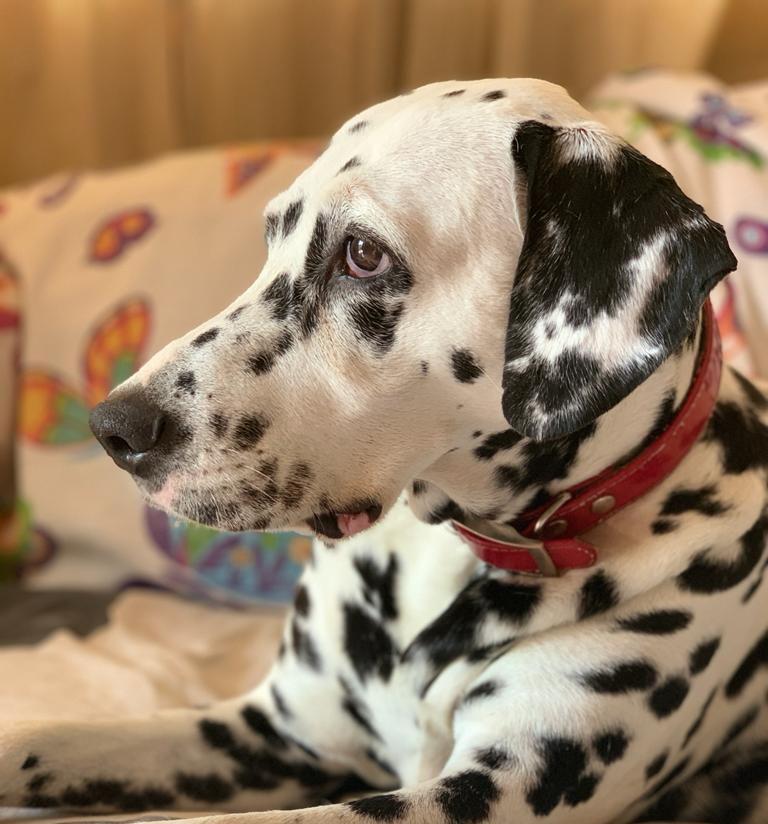
\includegraphics[
  width=0.6\textwidth]{khaleesi.jpg}

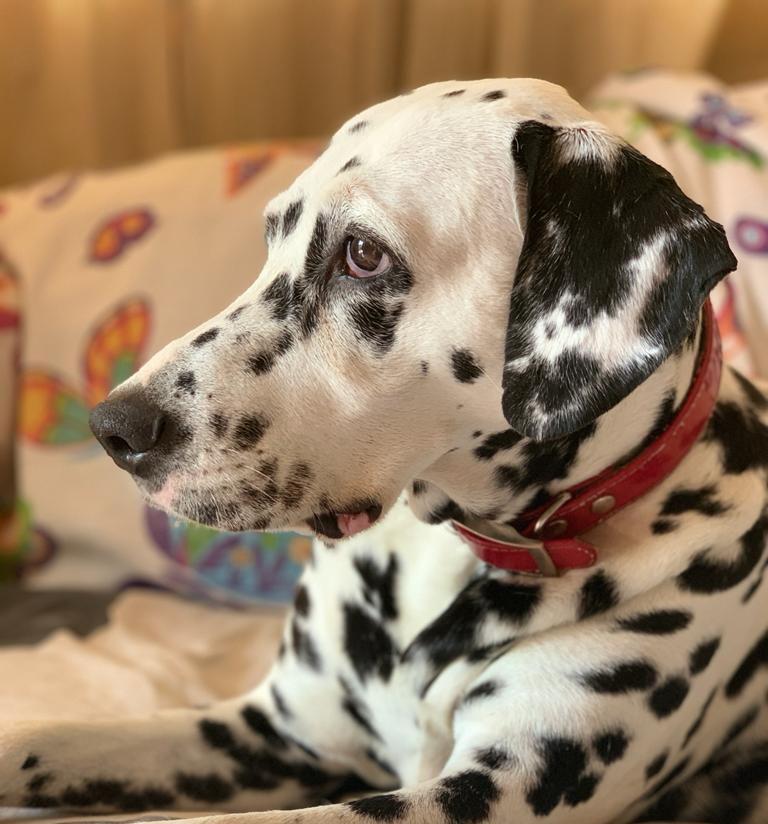
\includegraphics[
  width=0.4\textwidth,
  height=0.4\textwidth,
  angle=30
  ]{khaleesi} % no cal posar el format
\end{exampletwouptiny}

\end{frame}

%%%%%%%%%%%%%%%%%%%%%%%%%%%%%%%%%%%%%%%%%%%%%%%%%%%%%%%%%%%%%%%%%%%%%%%%%%%%%%%
%%%%%%%%%%%%%%%%%%%%%%%%%%%%%%%%%%%%%%%%%%%%%%%%%%%%%%%%%%%%%%%%%%%%%%%%%%%%%%%
%%%%%%%%%%%%%%%%%%%%%%%%%%%%%%%%%%%%%%%%%%%%%%%%%%%%%%%%%%%%%%%%%%%%%%%%%%%%%%%
\begin{frame}[fragile]{Incís: Aruments Opcionals}
\begin{itemize}
\item Fem servir claudàtors \keystrokebftt{[} \keystrokebftt{]} per arguments opcionals,
en comptes de claus \keystrokebftt{\{} \keystrokebftt{\}}.
\item \cmdbs{includegraphics} admet arguments opcionals per modificar la imatge.
Per exemple, \bftt{width=0.3\cmdbs{textwidth}} fa que la image ocupi un 30\% de l'amplada
del text (\cmdbs{textwidth}).
\item \cmdbs{documentclass} també admet arguments opcionals. Exemple:
\mint{latex}|\documentclass[12pt,twocolumn]{article}|
augmenta el tamany de text (12pt) i fa servir 2 columnes (molt típic d'articles acadèmics).
\item Com sabem quins arguments opcionals té una ordre? Cal buscar-ho a la documentació dels paquets.
Més endevant veurem com es fa.
\end{itemize}
\end{frame}

%%%%%%%%%%%%%%%%%%%%%%%%%%%%%%%%%%%%%%%%%%%%%%%%%%%%%%%%%%%%%%%%%%%%%%%%%%%%%%%
%%%%%%%%%%%%%%%%%%%%%%%%%%%%%%%%%%%%%%%%%%%%%%%%%%%%%%%%%%%%%%%%%%%%%%%%%%%%%%%
%%%%%%%%%%%%%%%%%%%%%%%%%%%%%%%%%%%%%%%%%%%%%%%%%%%%%%%%%%%%%%%%%%%%%%%%%%%%%%%
\subsection[fragile]{Floats}
\begin{frame}{Floats}
\begin{itemize}
\item Deixa que \LaTeX{} decideixi on posar la figura (pot ``flotar'').
\item En documents acadèmics caldrà afegir un peu de foto.
\item També se li pot donar una etiqueta amb \cmdbs{label}, que ens permetrà referir-nos a la figura amb \cmdbs{ref}.
\end{itemize}
\begin{minipage}{0.55\linewidth}
\inputminted[fontsize=\scriptsize,frame=single,resetmargins]{latex}%
  {media-graphics.tex}
\end{minipage}
\begin{minipage}{0.35\linewidth}
\includegraphics[width=\textwidth,clip,trim=2in 5in 3in 1in]{media-graphics.pdf}
\end{minipage}
\end{frame}

%%%%%%%%%%%%%%%%%%%%%%%%%%%%%%%%%%%%%%%%%%%%%%%%%%%%%%%%%%%%%%%%%%%%%%%%%%%%%%%
%%%%%%%%%%%%%%%%%%%%%%%%%%%%%%%%%%%%%%%%%%%%%%%%%%%%%%%%%%%%%%%%%%%%%%%%%%%%%%%
%%%%%%%%%%%%%%%%%%%%%%%%%%%%%%%%%%%%%%%%%%%%%%%%%%%%%%%%%%%%%%%%%%%%%%%%%%%%%%%
\begin{frame}[fragile]{Floats 2}
\begin{itemize}
\item Les opcions h (here), t (top), b (bottom), p (page) permeten indicar aproximadament on es vol el \textit{float} a la pàgina.
\item Es poden combinar: l'odre de preferència es $h > t > p> b$
\item Més informació a \href{https://www.overleaf.com/latex/examples/understanding-floats/qkjpvqptqrwd}{aquest tutorial en anglès, i les seves referències}.
\end{itemize}
\begin{exampletwouptiny}
\begin{figure}[htbp]
\centering

\includegraphics[
width=0.5\textwidth]{khaleesi2}
\end{figure}
\end{exampletwouptiny}

\end{frame}

%%%%%%%%%%%%%%%%%%%%%%%%%%%%%%%%%%%%%%%%%%%%%%%%%%%%%%%%%%%%%%%%%%%%%%%%%%%%%%%
%%%%%%%%%%%%%%%%%%%%%%%%%%%%%%%%%%%%%%%%%%%%%%%%%%%%%%%%%%%%%%%%%%%%%%%%%%%%%%%
%%%%%%%%%%%%%%%%%%%%%%%%%%%%%%%%%%%%%%%%%%%%%%%%%%%%%%%%%%%%%%%%%%%%%%%%%%%%%%%
\subsection{Taules}
\begin{frame}[fragile]{Taules}
\begin{itemize}
\item Les taules amb \LaTeX{} són una mica complexes.
\item Cal el paquet \bftt{tabularx}.
\item L'argument especifica l'alineament de les columnes --- \textbf{l}eft, \textbf{c}enter, \textbf{r}ight.
\begin{exampletwouptiny2}
\begin{tabular}{lcr}
    Item      & Num & Preu \$ \\
    Pantalla  & 1   & 199.99  \\
    Ordinador & 2   & 399.99  \\
    Cables    & 3   & 19.99   \\
\end{tabular}
\end{exampletwouptiny2}
\item \keystrokebftt{\&} marca el separador de columna i \keystrokebftt{\bs\bs} el final de línia.
\begin{exampletwouptiny2}
\begin{table}
    \centering % centra la taula
    \caption{Descriu preus.}
    \begin{tabular}{lcr}
        Item      & Num & Preu \$ \\
        Pantalla  & 1   & 199.99  \\
        Ordinador & 2   & 399.99  \\
        Cables    & 3   & 19.99   \\
    \end{tabular}
    \label{taula:items}
\end{table}
\end{exampletwouptiny2}
\end{itemize}
\end{frame}

%%%%%%%%%%%%%%%%%%%%%%%%%%%%%%%%%%%%%%%%%%%%%%%%%%%%%%%%%%%%%%%%%%%%%%%%%%%%%%%
%%%%%%%%%%%%%%%%%%%%%%%%%%%%%%%%%%%%%%%%%%%%%%%%%%%%%%%%%%%%%%%%%%%%%%%%%%%%%%%
%%%%%%%%%%%%%%%%%%%%%%%%%%%%%%%%%%%%%%%%%%%%%%%%%%%%%%%%%%%%%%%%%%%%%%%%%%%%%%%
\begin{frame}[fragile]{Taules 2}
\begin{itemize}
\item Els separadors \keystrokebftt{|} dins l'argument fan línies verticals (millor evitar-les),\\
\cmdbs{hline} fa línies horizontals.
\begin{exampletwouptiny}
\begin{tabular}{|l|r|r|}
    \hline
    Item      & Num & Preu \$ \\
    \hline
    Pantalla  & 1   & 199.99  \\
    Ordinador & 2   & 399.99  \\
    Cables    & 3   & 19.99   \\
    \hline
\end{tabular}
\end{exampletwouptiny}
\item El paquet \bftt{booktabs} proporciona les ordres \cmdbs{toprule}, \cmdbs{midrule} i \cmdbs{bottomrule}.
\begin{exampletwouptiny}
\begin{tabular}{lrr}
    \toprule
    Item      & Num & Preu \$ \\
    \midrule
    Pantalla  & 1   & 199.99  \\
    Ordinador & 2   & 399.99  \\
    Cables    & 3   & 19.99   \\
    \bottomrule
\end{tabular}
\end{exampletwouptiny}
\end{itemize}
\end{frame}

%%%%%%%%%%%%%%%%%%%%%%%%%%%%%%%%%%%%%%%%%%%%%%%%%%%%%%%%%%%%%%%%%%%%%%%%%%%%%%%
%%%%%%%%%%%%%%%%%%%%%%%%%%%%%%%%%%%%%%%%%%%%%%%%%%%%%%%%%%%%%%%%%%%%%%%%%%%%%%%
%%%%%%%%%%%%%%%%%%%%%%%%%%%%%%%%%%%%%%%%%%%%%%%%%%%%%%%%%%%%%%%%%%%%%%%%%%%%%%%
\begin{frame}[fragile]{Taules 3}
Hi ha moltes opcions diferents per fer taules.
\begin{itemize}
\item Es poden fusionar columnes amb \cmdbs{multicolumn} i files amb \cmdbs{multirow} (cal el paquet \bftt{multirow}).
\item Línies horitzontals més curtes amb \cmdbs{cline} o \cmdbs{cmidrule} de \bftt{booktabs}.

\begin{exampletwouptiny}
\begin{tabular}{lrr}
\toprule
Item &
\multicolumn{2}{c}{MultiColumna} \\
\cline{2-3}
Pantalla  & 1   & 199.99  \\
\cmidrule{1-2}
\multirow{2}{*}{MultiFila} & 2 & 3.99\\
& 3   & 19.99   \\
\bottomrule
\end{tabular}
\end{exampletwouptiny}
\end{itemize}
\end{frame}


%%%%%%%%%%%%%%%%%%%%%%%%%%%%%%%%%%%%%%%%%%%%%%%%%%%%%%%%%%%%%%%%%%%%%%%%%%%%%%%
%%%%%%%%%%%%%%%%%%%%%%%%%%%%%%%%%%%%%%%%%%%%%%%%%%%%%%%%%%%%%%%%%%%%%%%%%%%%%%%
%%%%%%%%%%%%%%%%%%%%%%%%%%%%%%%%%%%%%%%%%%%%%%%%%%%%%%%%%%%%%%%%%%%%%%%%%%%%%%%
\begin{frame}{Final de la primera part}
\begin{itemize}
\item Ja hem aprés a \dots
\begin{itemize}
\item Escriure text amb \LaTeX.
\item Utilitzar diferents ordres.
\item Tractar errors quan apareixen.
\item Escriure matemàtiques.
\item Utilitzar diversos entorns diferents.
\item Carregar paquets.
\item Mostrar figures i taules.
\end{itemize}
\item A la segona part, veurem com utilitzar \LaTeX{} per escriure documents amb seccions, referències creuades i bibliografia. Fins llavors!
\end{itemize}
\end{frame}

\begin{frame}{Referències en línia}
\begin{itemize}
\item \href{https://www.overleaf.com/learn}{The Overleaf Learn Wiki} --- tutorials i material de referència.
\item \href{http://en.wikibooks.org/wiki/LaTeX}{The \LaTeX{} Wikibook} --- més tutorials i material de referència.
\item \href{http://tex.stackexchange.com/}{\TeX{} Stack Exchange} --- preguntes i respostes
\item \href{http://www.latex-community.org/}{\LaTeX{} Community} --- fòrum
\item \href{http://ctan.org/}{Comprehensive \TeX{} Archive Network (CTAN)} --- documentació de paquets.
\item Qualsevol buscador us portarà a alguna d'aquestes pàgines.
\end{itemize}

Repositori del curs: \href{https://github.com/Pastells/curs-latex}{Pastells/curs-latex}

\end{frame}

\end{document}
